%!TEX root = ../Thesis.tex
\chapter{Crosstalk Experiments}
\label{chap:experiments}
In this section we discuss the details of thorough experiments that we conducted in order to quantify how the crosstalk affects the perceived depth. For the sake of completeness, we performed various experiments on considerably complex (realistic looking) rendered images that consisted of stimuli of various widths and geometric complexities. The effect of crosstalk were observed for both stereoscopic and automultiscopic displays.

\section{Motivation}
Even though previously some work has been done by Tsirlin \cite{tsirlin2011effect}\cite{tsirlin2012crosstalk}\cite{tsirlin2012effect} in order to understand these effects, we \textcolor{red}{felt that the experiments were incomplete and needed some more thorough investigation.}. The reason for that is that firstly Tsirlin's experiments were performed on monochromatic images where no other depth cue other than disparity was present. As mentioned in chapter 3, we conducted such a pilot experiment on ourselves (the author and one colleague) with a thin rectangular white bar on a black background using a similar Wheatstone setup and found that it took some getting used to to sense any depth of the stimulus even at high disparities. Even after spending some time on it, it was extremely hard and unreliable to guess the apparent distance of the stimulus from the screen in length units. This would mean that the naive test subjects would also have encountered the same problems. This observation is backed by the fact that the test subjects in \cite{tsirlin2012effect} and \cite{tsirlin2011effect} reported reduced depth of the stimuli even when no crosstalk was present. More reliable experiments would be ones where the test subjects report the actual theoretical depth in the base case i.e. when no crosstalk is present. Coupled with the fact that the test subjects were simply asked to report the perceived depth via a sliding bar representing zero or some maximum depth at extremes of the bar, it is likely that generated results could have been unreliable. The scenes of the natural world usually have at least some other monocular cues e.g. proper light shading, texture gradients and defocus blur etc. Moreover, since one factor contributing to visibility of the ghosts is also how much it is separated from the object, wide objects at some disparity will exhibit less visible ghosting than thin stimuli.

It is commonly believed that the reason for degraded observed depth in the presence of crosstalk is due to the fact that the human visual system is confused in choosing the correct location (or disparity) of the correct match for an object in the corresponding binocular retinal image. To the best of our knowledge, it is yet unclear whether this HVS confusion is elevated or reduced when the geometric complexity of the object (stimulus) is increased.  Which is why we thought it would be important to understand the relation of crosstalk on observed depth on stimuli of different widths and geometric complexities. Current studies suggests that for a certain crosstalk level and considerably smaller width of a desperate object, the extent of observed depth degradation increases as the disparity increase. This sounds counter-intuitive because for substantially high disparity of a thin object, the ghost will be completely separated and far away from the actual object itself. If the reason for degraded depth is actually the confusion of HVS in finding the proper match, then in such case the HVS should be able to find the proper match relatively easily because it is easy to distinguish between the ghost and the object as compared to the case of overlapping ghost. We hypothesized that the observed depth of any object with respect to the actual theoretical depth should degrade as long as some part of the ghost overlaps the object itself and the observed depth should improve when the ghost completely separates. Hence the graphs of figure \ref{fig:tsirlin_res} should be \say{U shaped}.

In stereoscopic displays, the arrangement of object-ghost pair is antisymmetric between the eyes \textcolor{red}{maybe make a diagram for this from the notebook}. This however is not the case with automultiscopic screens. As seen in figure \ref{fig:gaussians}, at least two of the neighboring views are responsible for adding crosstalk at any view point. Also, at the sweet spots, the number of views involved in light leakage from the left is always equal to the number of light leaking views from the right. Because the automultiscopic screen displays light fields, the arrangement of object-ghost tuple is symmetric in both eyes (at sweet spots). The HVS might react differently to this major difference. Again, to the best of our knowledge, until now there have been no studies that observed the effect of crosstalk on perceived depth in automultiscopic displays.\pagebreak

\section{stimuli}
Our stimuli consisted of an object (cylinder or a dragon) placed in front of a plane that had a light wooded texture. The reason for choosing a textured background was the HVS's efficiency in distinguishing between textures. This would make it easy for the observer to correctly guess the distance between the background and the foreground object. In order to make sure that our stimuli contains most of the basic monocular cues, we properly rendered them on computer using blender 2.73.
The blender scene as shown in figure \ref{fig:blender_scene} consisted of a an object of interest placed at origin. The background plane with wooden texture was placed 3 meters (world units) behind the object parallel to the camera plane. In order to capture the shading effects on the object, the scene was lit with a light source (sun) that was placed 10 meters in front and 3 meters at height of the object. Finally the camera was 10 meters in front of the object. The stereo scene was generated by capturing the two images at some distance on each side parallel to the image plane. This distance represented the baseline of the cameras.

Our experiments were based on test subjects judging the observed distance between the cylinder and the textured plane. This could have been achieved by either moving the cylinder or by moving the background plane in space relative to the camera. This however would have changed the object or the texture size which could have been used as a cue by the observers. In order to avoid that, we simply generated a dense series of images with varying camera baselines and keeping the position of the background plane in lock with respect to the camera. This way, the background was always at zero disparity (i.e. the plane of focus) and the cylinder always had a crossed disparity meaning the cylinder always appeared to be in front of the plane by some distance. In order to avoid resizing, images were rendered at the resolution of 768x432. With the smallest baseline, the observed distance between the cylinder and the plane was negligible where as this distance appeared to be increasing as the baseline increased all while keeping the size of object, size of texture and the proximity of the object to the texture constant. For the objects we chose four cylinders of different radii and a dragon from Stanford's 3D scanning repository. The details of each of those objects can be found in table \ref{tab:stimili_desc}.
\begin{table}[h!]
  \begin{center}
    \caption{Description of objects used as stimuli.}
    \label{tab:stimili_desc}
    \begin{tabular}{ccc}
      \toprule
      Object & Scene Dimensions (xyz) & Rendered Dimensions (arcmin)\\
      \midrule
      Cylinder(thin) & 5cm x 2m x 5cm & 18.9\\
      Cylinder(medium) & 10cm x 2m x 10cm & 37.8\\
      Cylinder(think) & 45cm x 2m x 45cm & 56.7\\
      Cylinder(thickest) & 80cm x 2m x 80cm & 75.6 \\
      Dragon & 0.31m x 0.22m x 14.17cm & 380 (max) \\
      \bottomrule
    \end{tabular}
  \end{center}
\end{table}
\begin{figure}
\centering
    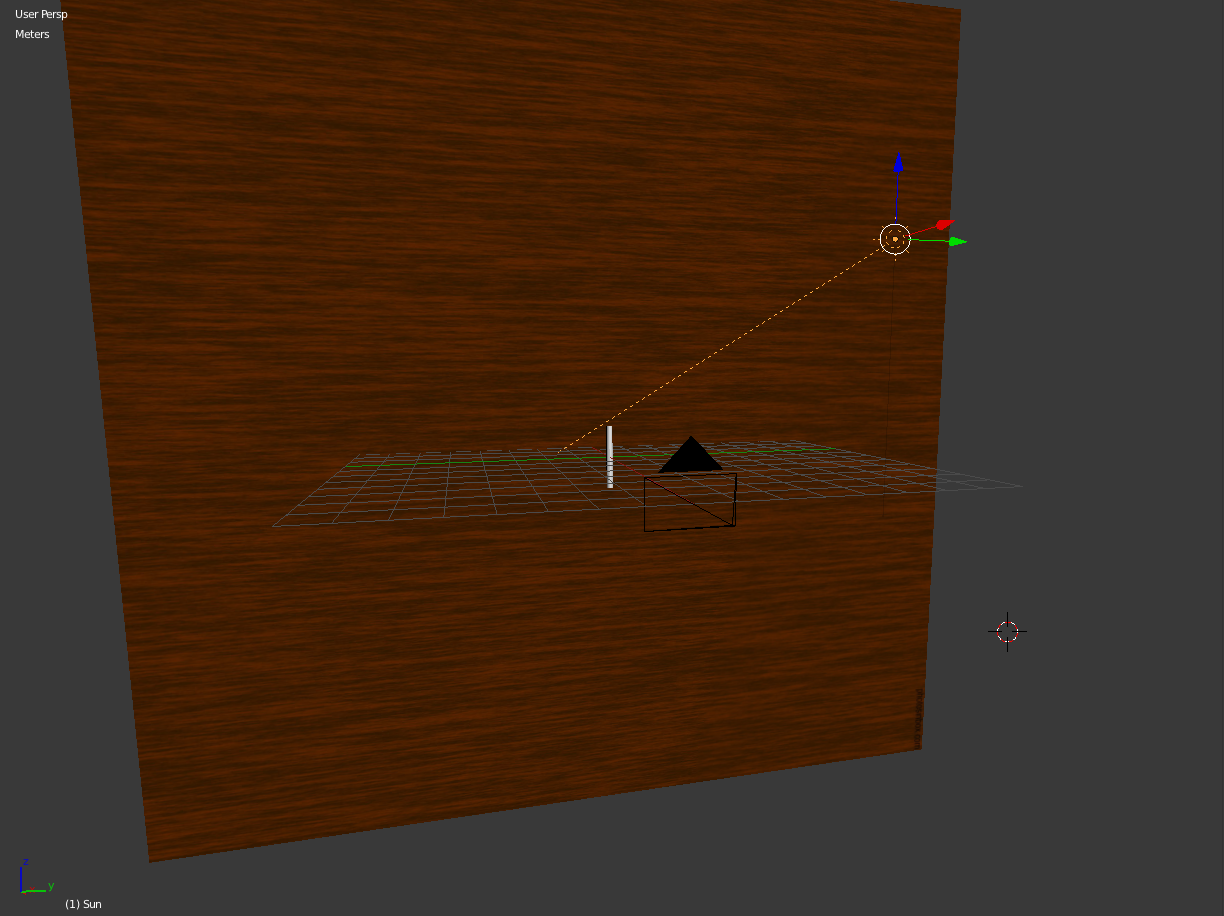
\includegraphics[width=0.5\textwidth]{./Template_Figures/blender_scene}
    \caption{Typical arrangement of the scene rendered with blender.\label{fig:blender_scene}}
\end{figure}

\subsection{Stereo and Automultiscopic stimuli}
For the stereo experiments, captured the scene with the camera baseline starting from 0.002 meters till 0.12 meters with the step of 0.002 meters. This gave us sixty sets of stereo images where the theoretical depth of the object of interest ranged from 0.04 cm to 3.45 cm (0-10.5 arcmins in terms of crossed disparity) in front of the plane of focus. Figure \ref{fig:stimuli_stereo} shows stereo images of one of the cylinder and the dragon. The step size was chosen small enough so that the transition from the minimum to the maximum depth for an object would seem continues to the observer.
\begin{figure}[htbp]
    % \centering
    \begin{subfigure}[b]{0.5\textwidth}
        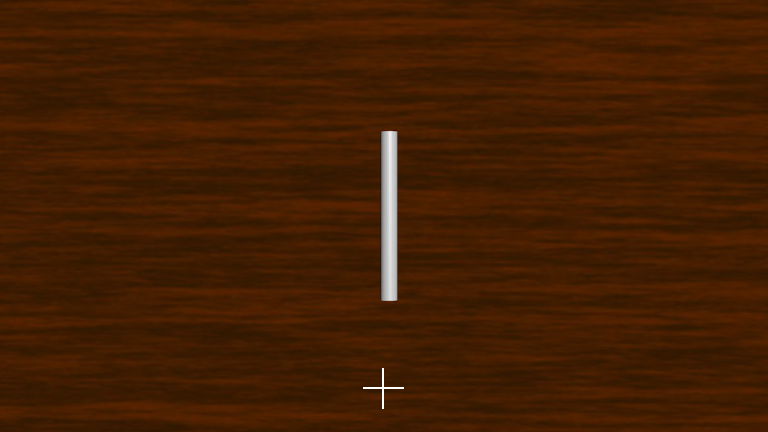
\includegraphics[width=\textwidth]{./Template_Figures/57L.png}
        \caption{}\label{fig:left_stereo_cyl}
    \end{subfigure}
    \begin{subfigure}[b]{0.5\textwidth}
        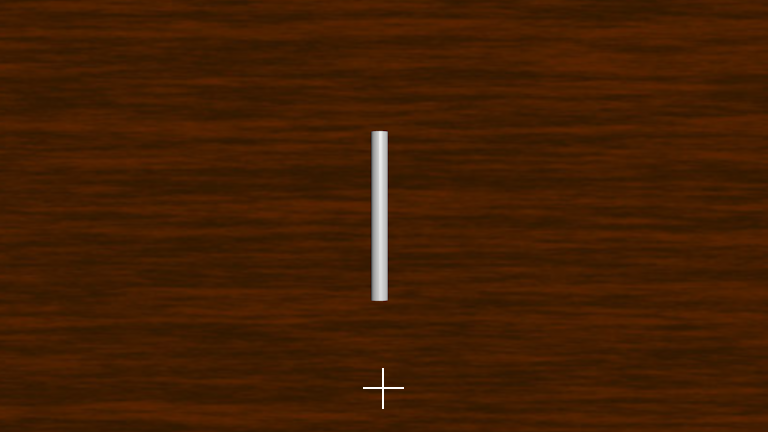
\includegraphics[width=\textwidth]{./Template_Figures/57R}
        \caption{}\label{fig:right_stereo_cyl}
    \end{subfigure}

    \begin{subfigure}[b]{0.5\textwidth}
        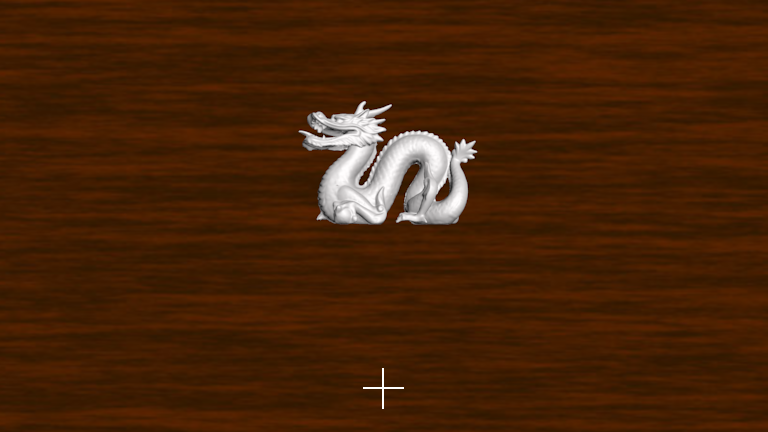
\includegraphics[width=\textwidth]{./Template_Figures/57Ld.png}
        \caption{}\label{fig:left_stereo_dra}
    \end{subfigure}
    \begin{subfigure}[b]{0.5\textwidth}
        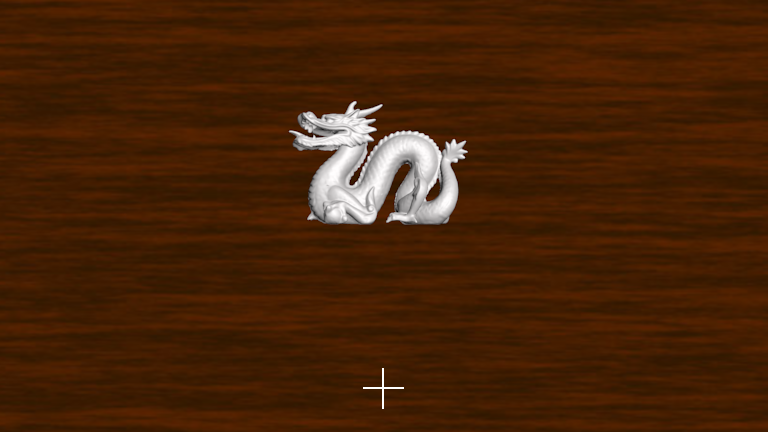
\includegraphics[width=\textwidth]{./Template_Figures/57Rd.png}
        \caption{}\label{fig:right_stereo_dra}
    \end{subfigure}
    \caption{Stereo images of the cylinder of 5 cm radius and the dragon. The theoretical depth difference between the objects and the background is 3.44 cm. Viewer can cross-fuse to see in depth.\label{fig:stimuli_stereo}}
\end{figure}

The images for automultiscopic experiments were rendered similarly. The only difference being that the range of baseline started from 0 until 0.24 meters. The reason for this is explained in the next section.

\section{Apparatus and simulation procedure}
The experiments were conducted on a commercial 47'' SIMS2 HDR47E LCD display with a resolution of 1920x1080. The left and right half of the screen each with a resolution of 960x1080 were gated to the left and right eye using a custom built Wheatstone setup \cite{ wiki:wheatstone} that consisted of two mirrors M1 and M2 set at $45^\circ$ angle with respect to the screen. The optical length from the eyes to the screen via mirrors M1 and M2 was measured at 87.3 cm. The whole setup was enclosed in a black box with an aperture through which the viewer could view the screen via mirrors M1. The display even though build for HDR viewing had a DVI plus mode for which the luminance measured with luminance meter via the aperture ranged from \textcolor{red}{?? to ??} $cdm^{-2}$. The DVI plus mode should (according to the documentation) mimic the traditional LCD display hence we chose to use this mode.
\begin{figure}[htbp]
    % \centering
    \begin{subfigure}[b]{0.5\textwidth}
        \includegraphics[width=\textwidth]{./Template_Figures/setup}
        \caption{}\label{fig:setup}
    \end{subfigure}
    \begin{subfigure}[b]{0.4\textwidth}
        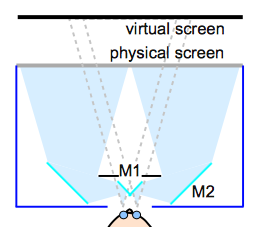
\includegraphics[width=\textwidth]{./Template_Figures/setup_sch}
        \caption{}\label{fig:setup_sch}
    \end{subfigure}
    \caption{Our Wheatstone setup. Physical view frusta are shaded in light blue where as the virtual view frusta are depicted in dotted gray lines. The cyan lines represent the mirrors \cite{vangorp2014depth}\label{fig:wheatstone_setup}}
\end{figure}

Since on an LCD panel, all the rgb channels equally and additively contribute to the crosstalk, we simulated the ghosted images simple by adding a percentage image of unintended view to the intended view image. For stereo, simple addition of a percentage of the right image into the left and vice versa sufficed. However, the automultiscopic case was a little tricky. First of all we simulated the view intensity profiles in figure \ref{fig:gaussians} using Gaussians with $\sigma = 2$ and means located at the sweet spots of the automultiscopic displays (figure \ref{fig:sim_gaussians}). To match the profiles in figure \ref{fig:gaussians}, the gaussians were upscaled such that the value 0.8 was attained at the mean. Using our simulated profiles, we found that at any sweet spot viewing position, the amount of light leaked from views other then the two adjacent views was negligible. Hence in our simulation we only considered light leakage from the adjacent views. Considering that an automultiscopic screen displays light fields sampled at frequency $1/\delta_x$ ($\delta_x$ being the step size at which the images were captured along the camera baseline), the leaked light from a position `y' to position `x' can be modeled as
\begin{equation}
l(y,x) \simeq a_y(x)\:.\:f(y)
\label{eq:ct_leak_eq}
\end{equation}
Where $a_y(x)$ is the Gaussian(corresponding to location y) value at position `x' and $f(y)$ is the light field image at position `y'. And the observe image \say{g} at any viewing position `x' can be mathematically modeled as
\begin{equation}
g(x) \: \simeq \: ...\: +\: l(x-2\delta_x,\:x)\:+\: l(x-\delta_x,\:x)\:+\:l(x,\:x)\:+\: l(x+2\delta_x,\:x)\:+\: l(x+\delta_x,\:x)\:+ \:...
\label{eq:ct_sim_eq}
\end{equation}
This would mean that the amount of ghost separation at any disparity of the object would be constant on either side. In order to keep the nature of the automultiscopic experiments similar to that of the stereo (where the ghost separation increase as the disparity increase), we changed the sampling rate $\delta_x$ with respect to the disparity of the object.
 \begin{figure}
\centering
    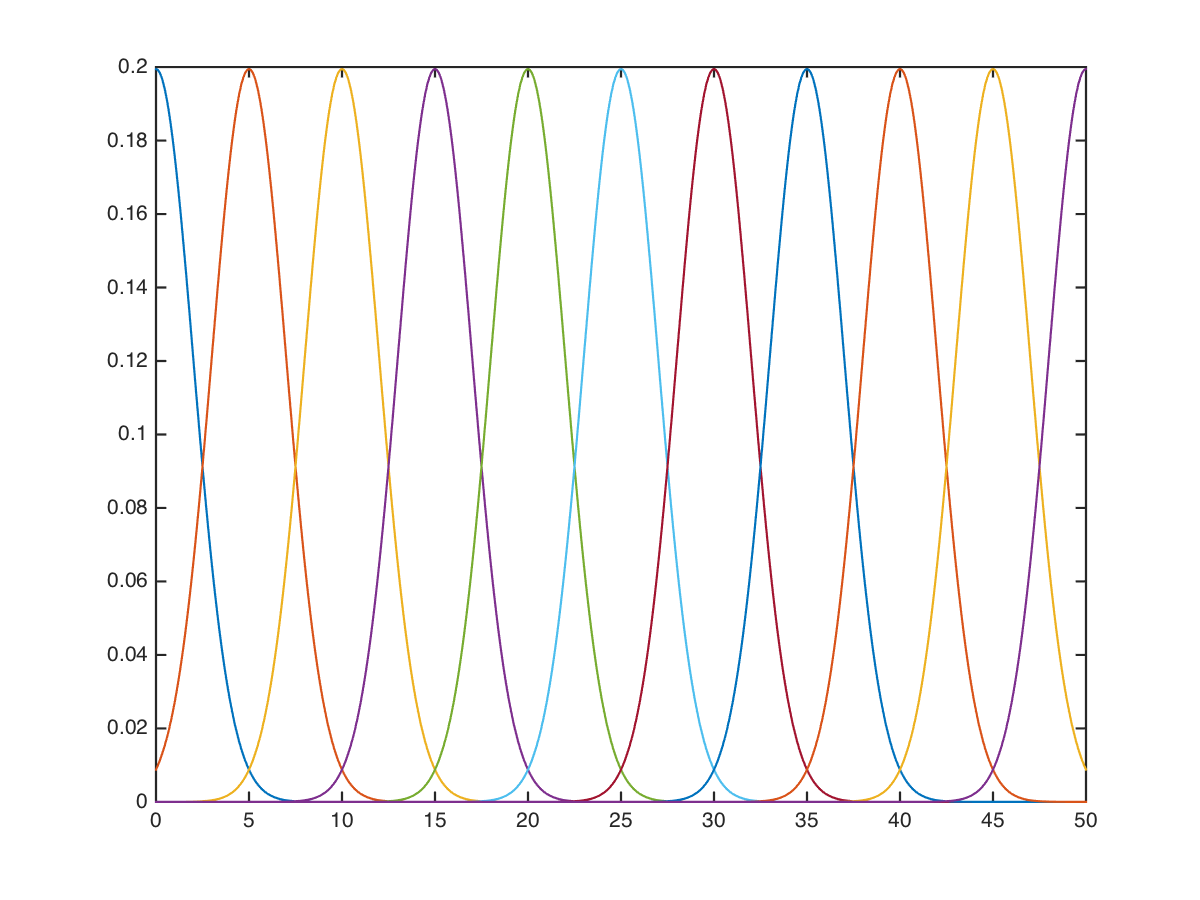
\includegraphics[width=0.7\textwidth]{./Template_Figures/sim_gaussians}
    \caption{Luminance intensity profiles for an 11 view automultiscopic display simulated with Gaussians of $\sigma =2$ centered at the sweet spots. X-axis denote the viewing position.\label{fig:sim_gaussians}}
\end{figure}
i.e. For a disparity `d', the the the observed left and right images can be written as
\begin{equation}
\begin{aligned}
g(d)_{left} \: \simeq l(2.d,\:d)\:+\: l(d,\:d)\:+\:l(0,\:d) \\
g(d)_{right} \: \simeq l(-2.d,\:-d)\:+\: l(-d,\:-d)\:+\:l(0,\:-d)
\end{aligned}
\label{eq:auto_obs_imgs}
\end{equation}
\begin{figure}[htbp]
    % \centering
    \begin{subfigure}[b]{0.5\textwidth}
        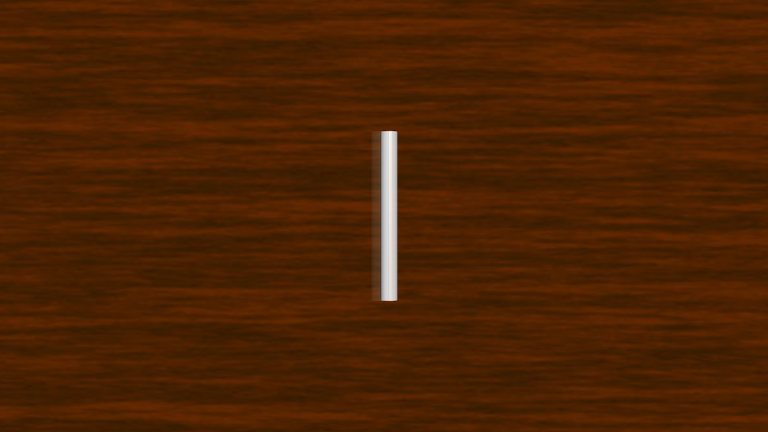
\includegraphics[width=\textwidth]{./Template_Figures/stereo_ghost_left}
        \caption{}\label{fig:obs_st_left}
    \end{subfigure}
    \begin{subfigure}[b]{0.5\textwidth}
        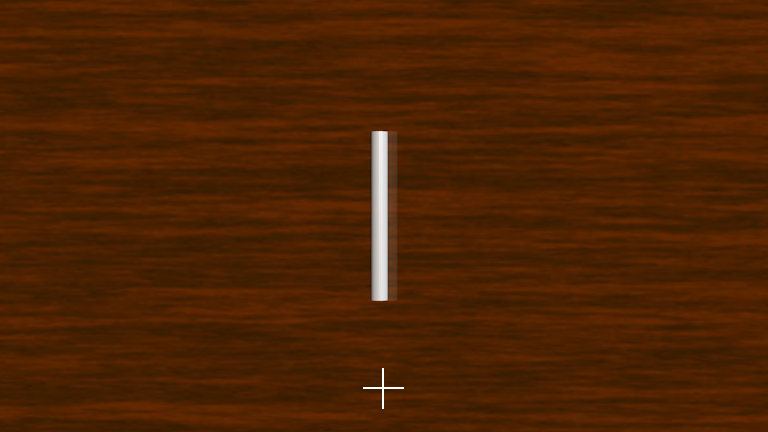
\includegraphics[width=\textwidth]{./Template_Figures/stereo_ghost_right}
        \caption{}\label{fig:obs_st_right}
    \end{subfigure}

    \begin{subfigure}[b]{0.5\textwidth}
        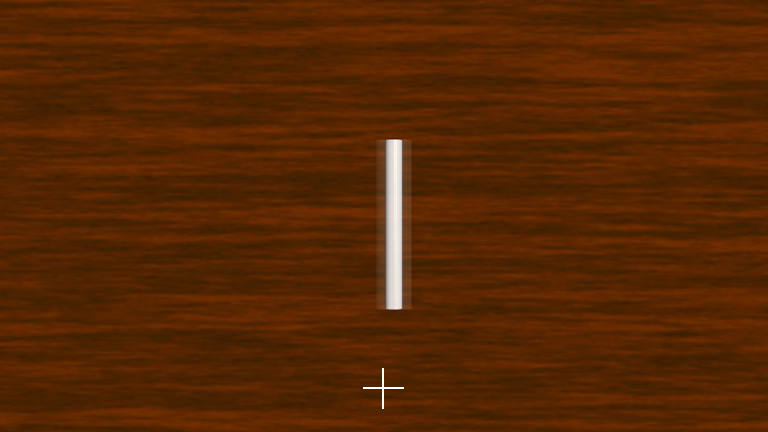
\includegraphics[width=\textwidth]{./Template_Figures/auto_ghost_left}
        \caption{}\label{fig:obs_aut_left}
    \end{subfigure}
    \begin{subfigure}[b]{0.5\textwidth}
        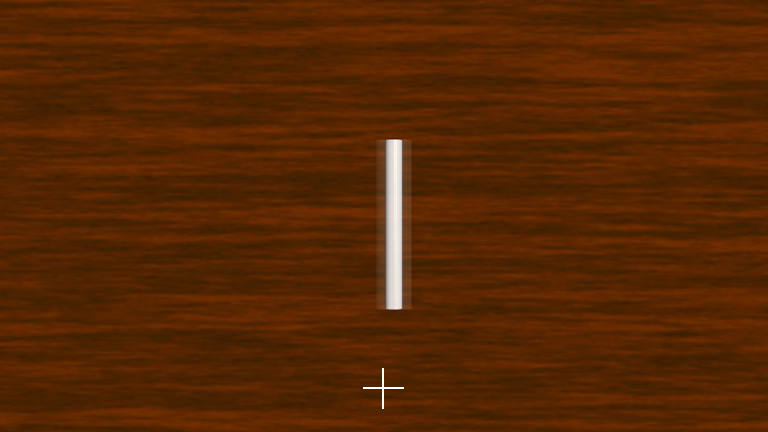
\includegraphics[width=\textwidth]{./Template_Figures/auto_ghost_left}
        \caption{}\label{fig:obs_aut_right}
    \end{subfigure}
    \caption{(a,b) Observed left and right stereo images with 14\% crosstalk and crossed depth of 3.45 cm. (c,d) Same configuration for observed images on automultiscopic display)\label{fig:observed_ct_images}}
\end{figure}

\section{Experiment procedure}
\subsection{Environment Setup}
For our experiments, we subdivided the screen horizontally, the upper half where the test subjects would see the crosstalk added scene(stimuli) with some fixed depth of the object, and the lower half where the subjects were shown the same scene without any crosstalk. We will refer to the upper half of the screen as reference stimulus and the lower half as test stimulus. Also we will call the depth difference between the background (wooden plane at zero disparity) and the foreground object (at some crossed disparity) the depth of the object. As mentioned in section 4.2, the depths of the object in the presented stimuli ranged from 0.04 to 3.45 centimeters. The subjects could vary the depth in the test stimulus in the above mentioned range via left and right mouse buttons. Due to the dense sampling of the light field (small baseline distance change), the change in the depth appeared continuous, i.e. the viewers could not observe any jumps while changing it. Pressing the left mouse button for 6 seconds would change the depth of the object from 0.04 cm to 3.45 cm, and vice versa for the right click. During the experiment, the subjects were tasked with matching the depth in the test stimulus to the observed depth of the reference. Upon matching the depth, the subjects would register the answer using the center mouse click. Figure \ref{fig:exp_env} shows the overall layout of the screen from a viewer's perspective. To avoid the possibility of the subject matching the absolute depths of the objects rather than the depth difference between the background plane and the object, as required, we shifted the depth of the reference stimulus by 3.45 cm towards the viewer whereas the depth of the test stimulus was shift equally away from the viewer. Thus ensuring that the depths of the objects would never coincide, and hence the subjects would not be able to match the absolute object's depth. In addition, a nonious cross-hair representing the plane of focus was added at the bottom center of the screen. Figure \ref{fig:exp_env_depth} shows the top view of the visualized environment. The experiment environment was created using Psychtoolbox-3 package for Matlab.
\begin{figure}[htbp]
    % \centering
    \begin{subfigure}[b]{0.65\textwidth}
        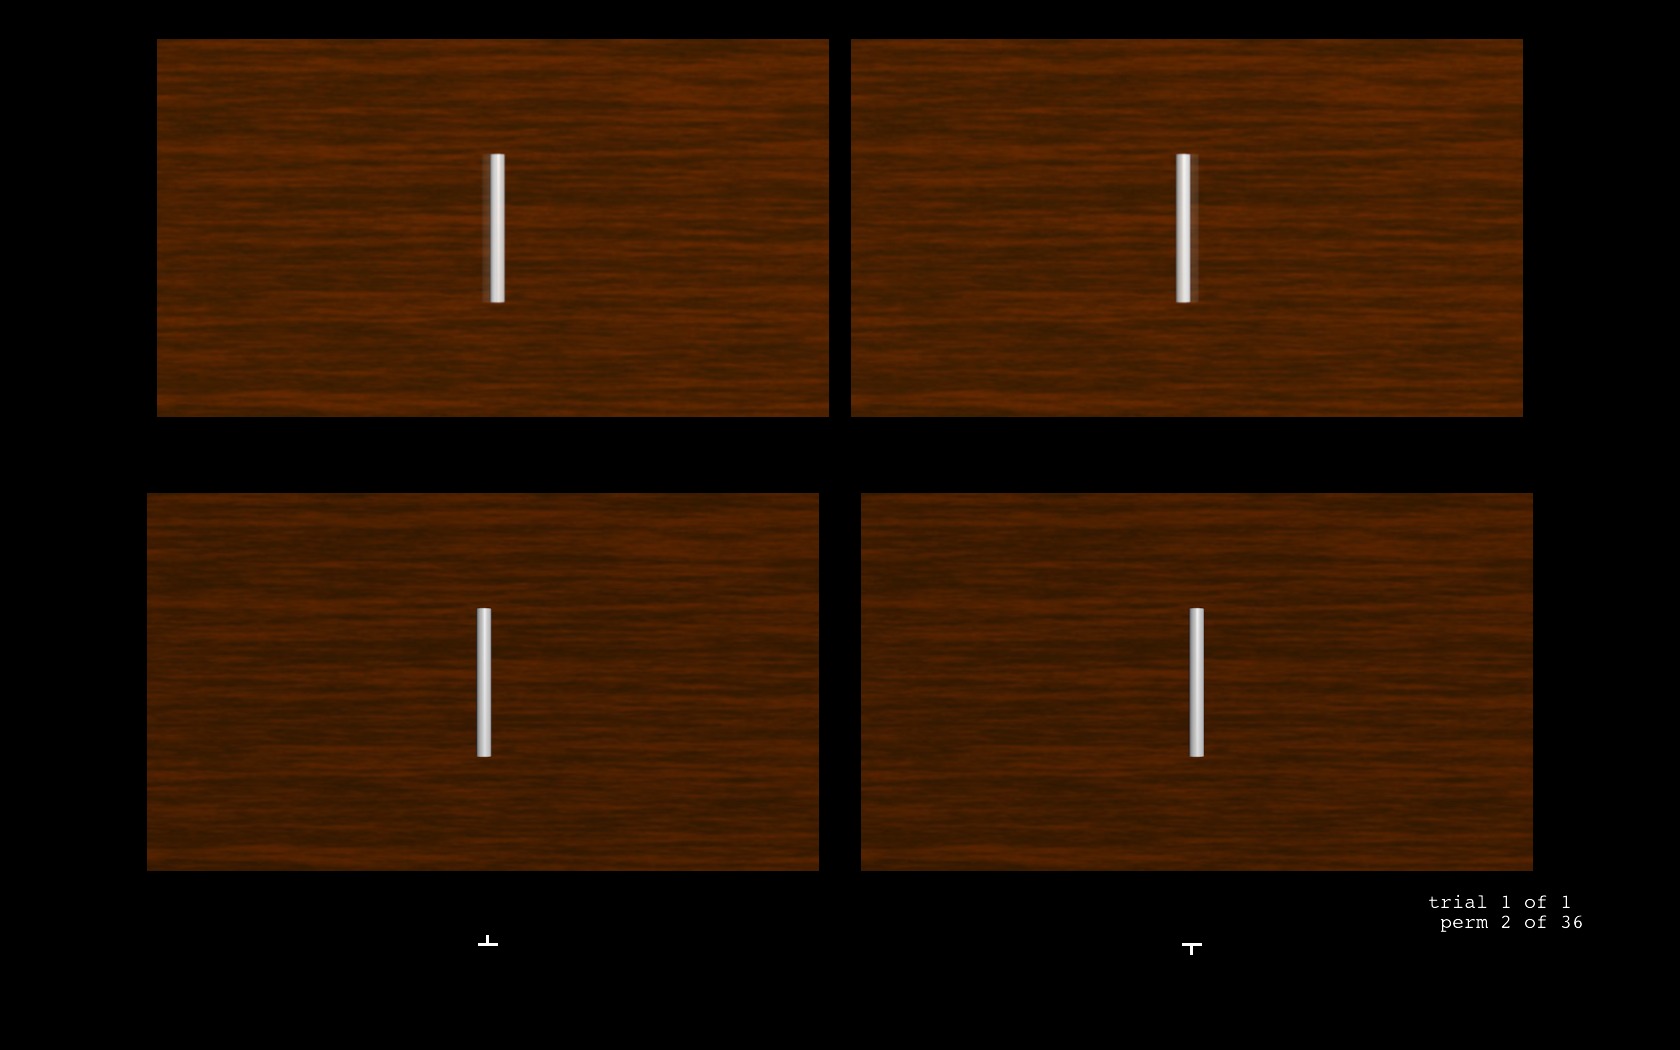
\includegraphics[width=\textwidth]{./Template_Figures/exp_env}
        \caption{}\label{fig:exp_env}
    \end{subfigure}
    \begin{subfigure}[b]{0.34\textwidth}
        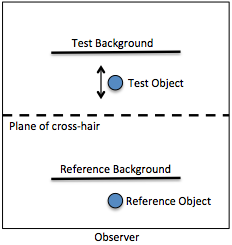
\includegraphics[width=\textwidth]{./Template_Figures/exp_env_depth}
        \caption{}\label{fig:exp_env_depth}
    \end{subfigure}

    \caption{(A) Schematics of the complete display. Upper half of the screen shows the reference stimulus with 14\% crosstalk. The bottom half shows the user controlled test stimulus free of crosstalk. (B) Layout of the experiment environment in terms of depth w.r.t. observer.\label{fig:exp_env_overall}}
\end{figure}

\subsection{Subjects}
Several paid test subjects and the author participated in the experiments. In order to ensure the subject's correctness of the stereo vision, they were first asked to identify the proximity of the test and reference stimuli with respect to the cross-hair. Also they were asked to identify the polarity of the change in depth of the test stimulus while the author changed it slightly in each direction. Table \ref{tab:agg_subj} shows the number of participants in each kind of experiments.
\begin{table}[ht!]
  \begin{center}
    \caption{Description of the number of subjects that participated in each experiment.}
    \label{tab:agg_subj}
    \begin{tabular}{ccc}
      \toprule
      Object & Stereo  & Automultiscopic\\
      \midrule
      Cylinder(thin) & 11 & 13  \\
      Cylinder(medium) & 11 & 11\\
      Cylinder(think) & 7 & 13\\
      Cylinder(thickest) & 8 & 13 \\
      Dragon & 13 & 13\\
      \bottomrule
    \end{tabular}
  \end{center}
\end{table}

\subsection{Experiment parameters}
Four levels of crosstalk i.e. 0\%, 3\%, 7\% and 14\% and seven levels of depths (crossed disparity) i.e. 0.04, 0.73, 1.18, 1.53, 1.75, 2.76 and 3.44 centimeters were chosen to be tested. We neglected any level of crosstalk greater than 14\% because in our pilot experiments we noticed that any greater crosstalk level almost always resulted in matching of the stimulus with the ghost resulting in total loss of depth. We couldn't find any commercial stereo display where the crosstalk levels were that high. Usually they are below 10\%. During the experiment, each subject was asked to match the observed depths for all possible combinations i.e 28 trials (4 crosstalk levels $\times$ 7 depth levels) in total for each kind of stimulus. Trials for stereoscopic and automultiscopic cases were conducted separately.
\\
\section{Results}

In the following section, median data for all the observers along with the standard error for each crosstalk level (figure \ref{fig:s_crosstalk_0} to ??) are shown. Individual lines in the graphs denote the different objects i.e. cylinders of all widths and the dragon as mentioned in table \ref{tab:stimili_desc}. The axis defines the actual and the observed theoretical disparity-defined depths. Ideally, all the graphs should be diagonally coinciding lines indicating no effect of crosstalk on perceived depth. Even though generally it is not the case, it can be observed that in the base case (no crosstalk), all the graphs (for all objects) almost approximates a diagonal line for both stereo and automultiscopic experiments. This is an improvement over \cite{tsirlin2012effect} meaning that the reported amounts of depth degradation for different cases would be more reliable.

\subsection{Stereo}
It can be seen in figure \ref{fig:s_crosstalk_0} that in absence of crosstalk, the observers mostly perceived the depths correctly. A slight overestimation of depth in case of the smallest depth (0.04 cm) can be seen for the thickest cylinder (width = 36 arcmin). Given the fact that the user controlled depth variation of test stimulus was continuous, it is reasonable to assume that it would be quite unlikely for the observers to exactly match the depths. Hence the slight overestimation of depth can be considered as an observer approximation error. The same however could not be straightforwardly said about the underestimation for the dragon at 2.76 cm depth which is mapped to approximately 2 cm observed depth. But since the next greater depth shows no underestimation, we can safely assume it to be a \textcolor{red}{human error}.
\begin{figure}[H]
\centering
    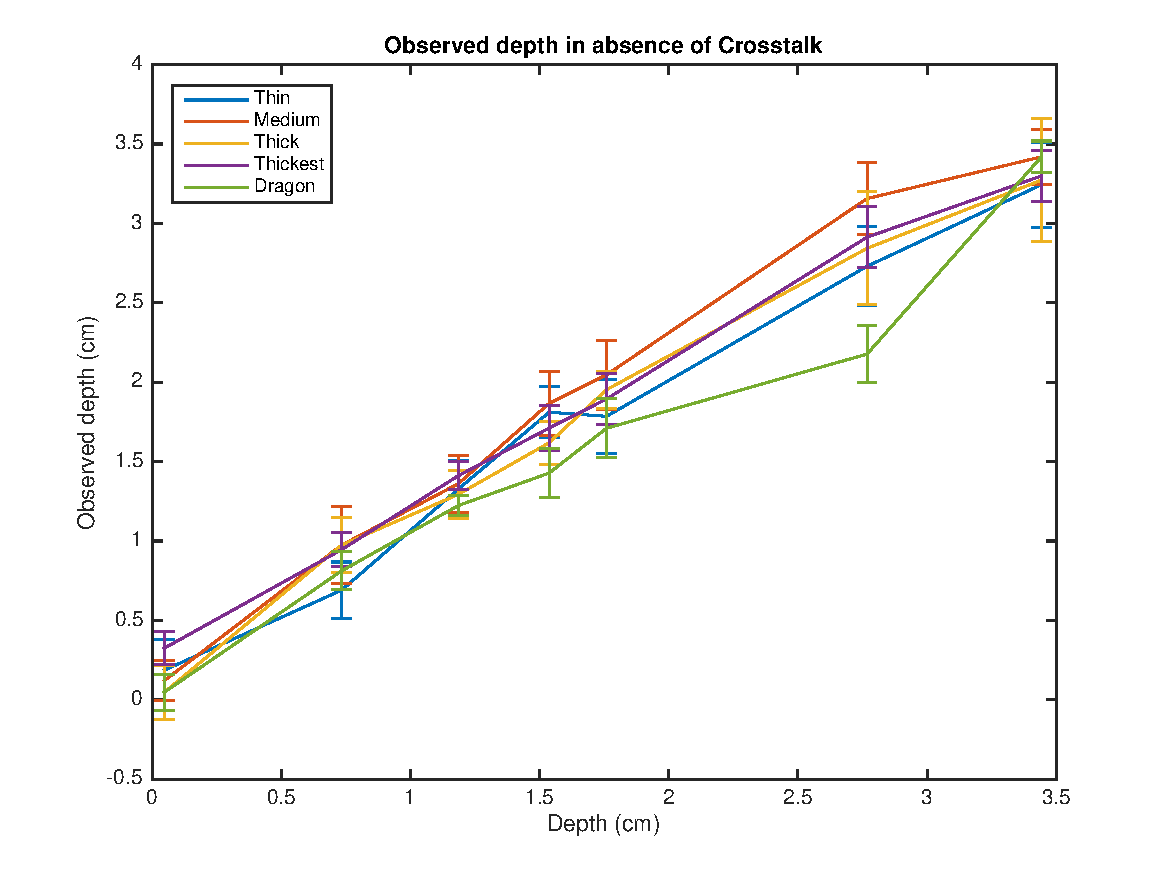
\includegraphics[width=0.9\textwidth]{./Template_Figures/s_crosstalk_0}
    \caption{Abscissa shows the observed depth when no crosstalk is present. The error bars indicate $\pm$ 1 standard error.\label{fig:s_crosstalk_0}}
\end{figure}

When the crosstalk is increased to 3\% (figure \ref{fig:s_crosstalk_3}), it is clear that the observed depth of thin(18.9 arcmin) cylinder starts degrading at depths greater than 1.75 cm. The angular disparity at this depth is 5.35 arcmin which would give the ghost separation of 28\%. A slight overestimation of the 2.76 cm depth for cylinder (75.6 arcmin) can be considered as approximation error. The reason for this again is that the next greater depth is observed without any degradation. We think it would be reasonable to consider this as a human approximation error because the HVS probably does not gets confused for some disparity and then behaves without any error for the following larger disparities. I.e. once the observed depth starts degrading at some disparity, provided all the other conditions are kept constant, it should keep on degrading for all larger disparities as well.
\begin{figure}[H]
\centering
    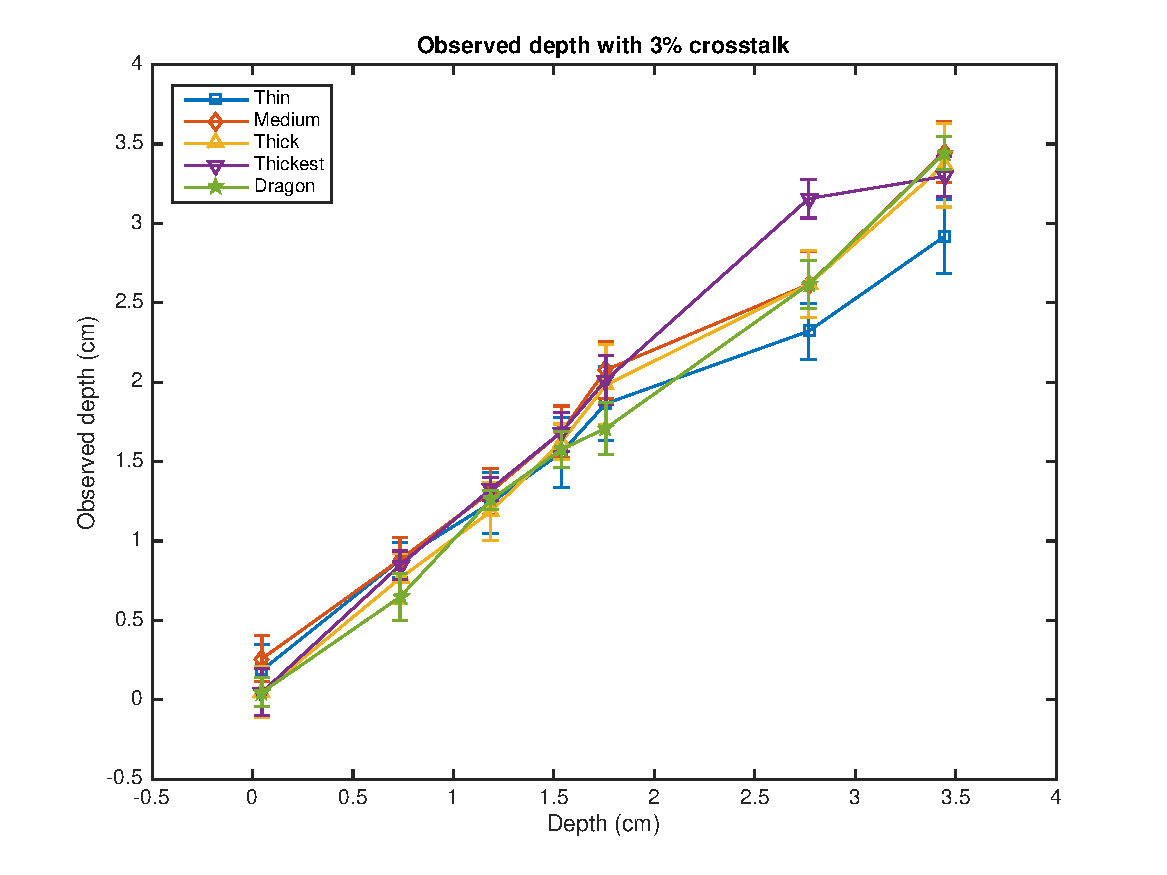
\includegraphics[width=0.9\textwidth]{./Template_Figures/s_crosstalk_3}
    \caption{Abscissa shows the observed depth when 3\% crosstalk is present. The error bars indicate $\pm$ 1 standard error.\label{fig:s_crosstalk_3}}
\end{figure}

Substantial effects on the observed depth starts appearing once the crosstalk level is increased to 7\% \ref{fig:s_crosstalk_7}. The cylinders of all widths show reduced observed depth. The reduction is most severe for the thin (18.9 arcmin) cylinder. The loss of observed depth appears to be lower as the width of the cylinder increases while the observed depth of the dragon seems to be unaffected. One interesting point to observe is that for all the cylinders, the perceived depth starts degrading at the actual depths of 1.75 cm or higher. For the thin cylinder, the ghost is completely separated only at the maximum i.e. 10.5 disparity arcmin. However the observed depth appears to be the same for the maximum and the second maximum i.e. 8.4 arcmin disparity. \textcolor{red}{why}. Also it should be noted that the graph for the thin cylinder shows signs of degradation even at actual depth of 1.13 cm.  The ghost separation at this point is ??\textcolor{red}{why also make a table of ghost separation}

Observed depth is severely affected for all the object once the crosstalk reaches 14\% \ref{fig:s_crosstalk_14}. The thin cylinder again shows signs of degradation starting at the actual depth of 1.13 cm where as the observed depths of all the other objects starts deteriorating at the theoretical depth of 1.76 cm. The pattern of wider objects showing less depth deterioration compared to thin objects is still observed. However, with such extreme crosstalk level, even the observed depth of the dragon is reported to be substantially affected.

\begin{figure}[H]
\centering
    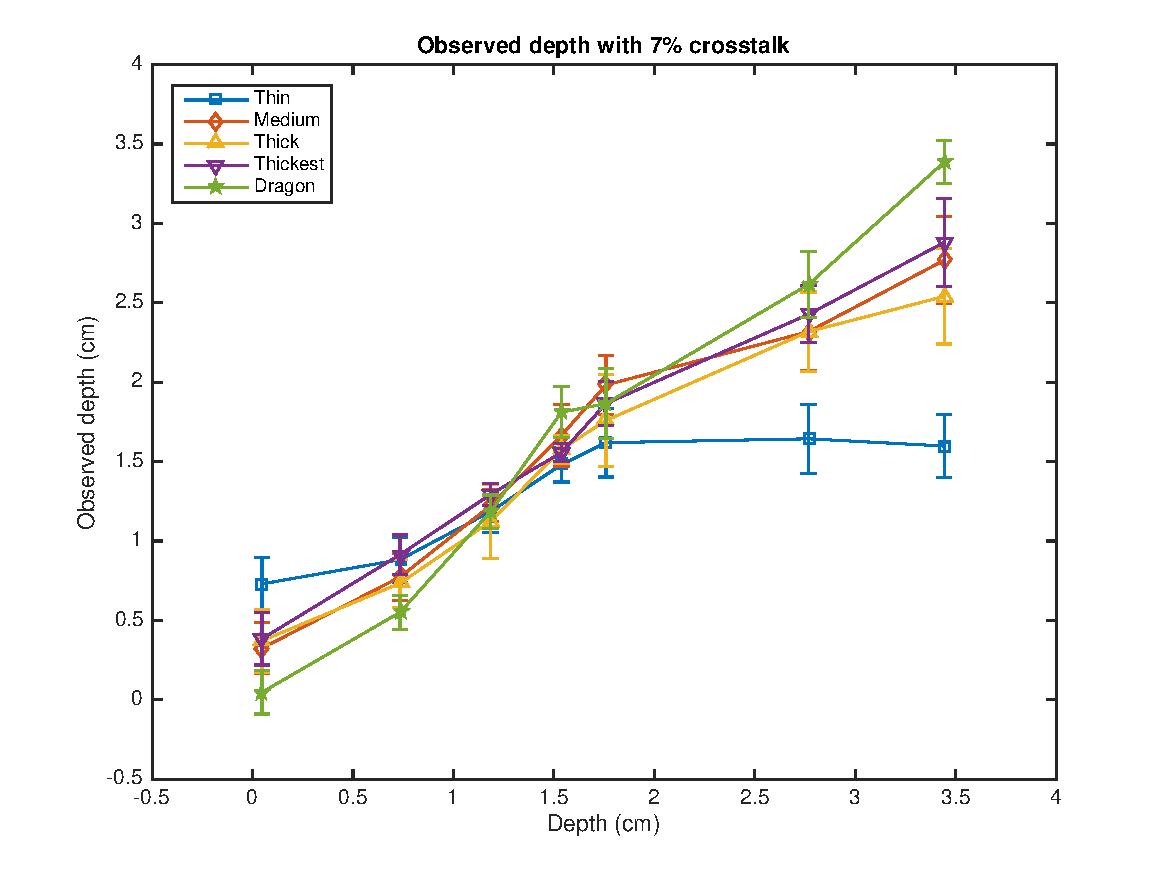
\includegraphics[width=0.9\textwidth]{./Template_Figures/s_crosstalk_7}
    \caption{Abscissa shows the observed depth when 7\% crosstalk is present. The error bars indicate $\pm$ 1 standard error.\label{fig:s_crosstalk_7}}
\end{figure}

\begin{figure}[H]
\centering
    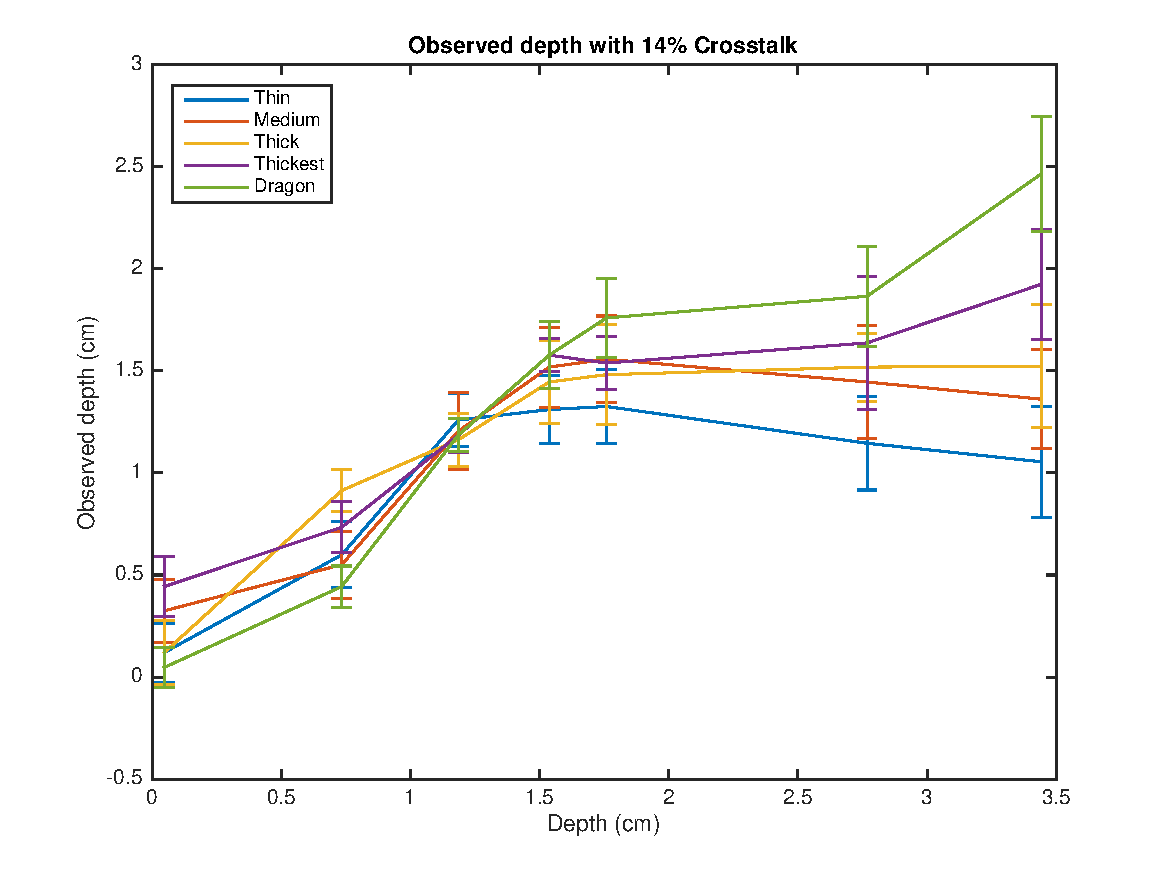
\includegraphics[width=0.9\textwidth]{./Template_Figures/s_crosstalk_14}
    \caption{Abscissa shows the observed depth when 14\% crosstalk is present. The error bars indicate $\pm$ 1 standard error.\label{fig:s_crosstalk_14}}
\end{figure}



\subsection{Automultiscopic}

\begin{figure}[H]
\centering
    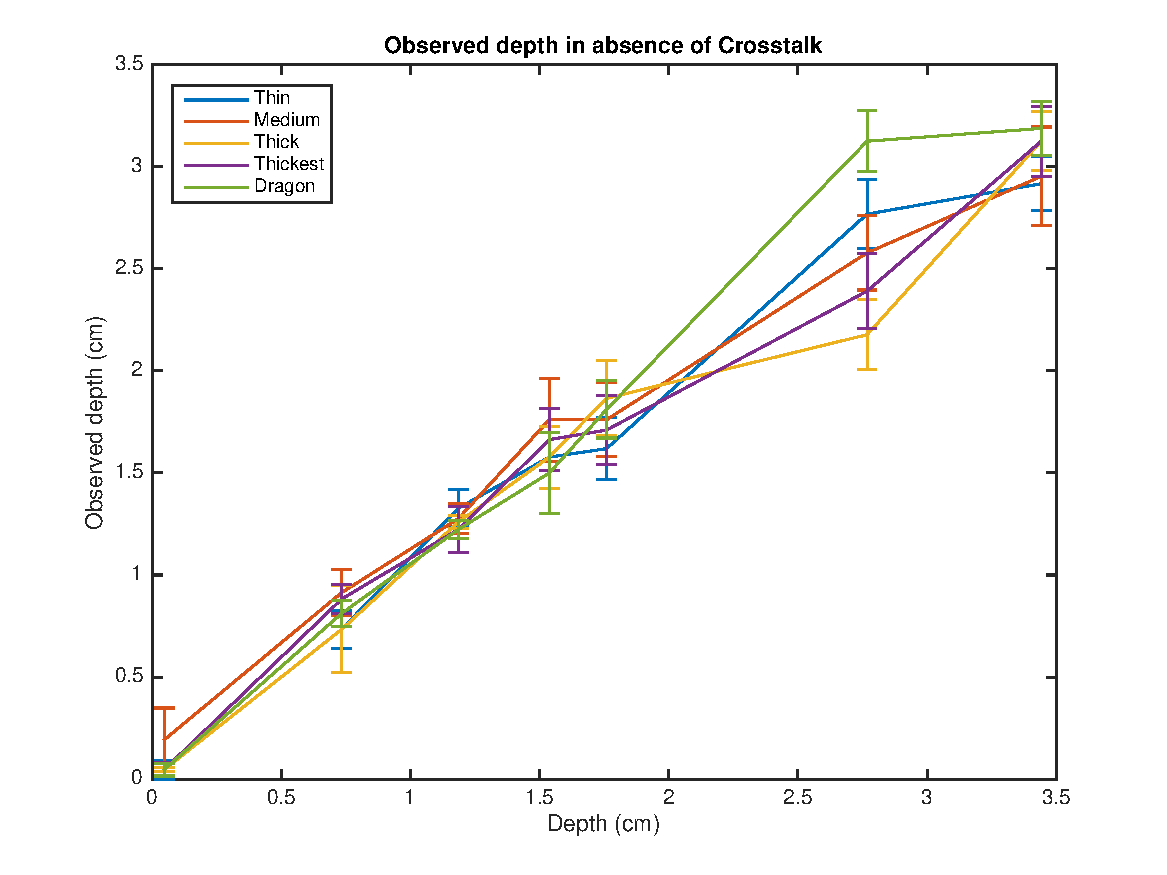
\includegraphics[width=0.9\textwidth]{./Template_Figures/a_crosstalk_0}
    \caption{Abscissa shows the observed depth when no crosstalk is present. The error bars indicate $\pm$ 1 standard error.\label{fig:a_crosstalk_0}}
\end{figure}

\begin{figure}[H]
\centering
    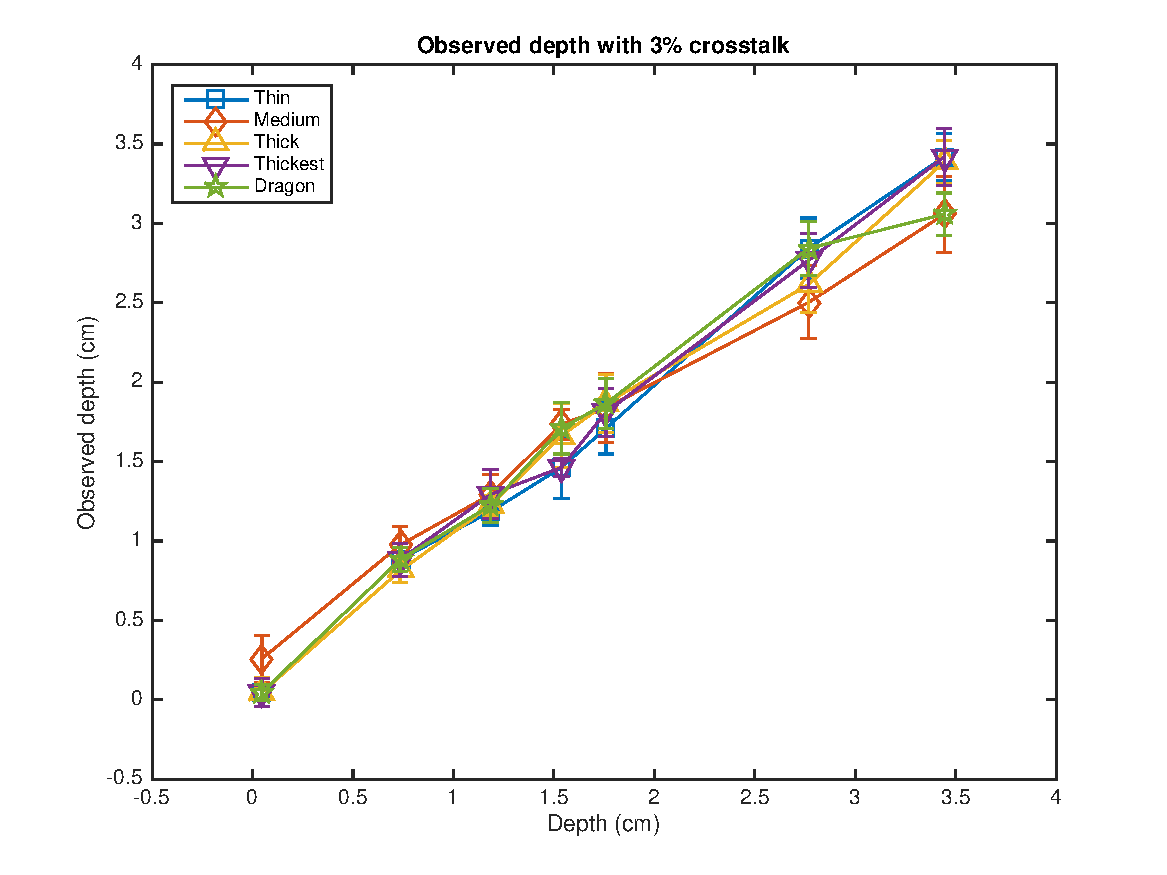
\includegraphics[width=0.9\textwidth]{./Template_Figures/a_crosstalk_3}
    \caption{Abscissa shows the observed depth when 3\% crosstalk is present. The error bars indicate $\pm$ 1 standard error.\label{fig:a_crosstalk_3}}
\end{figure}

\begin{figure}[H]
\centering
    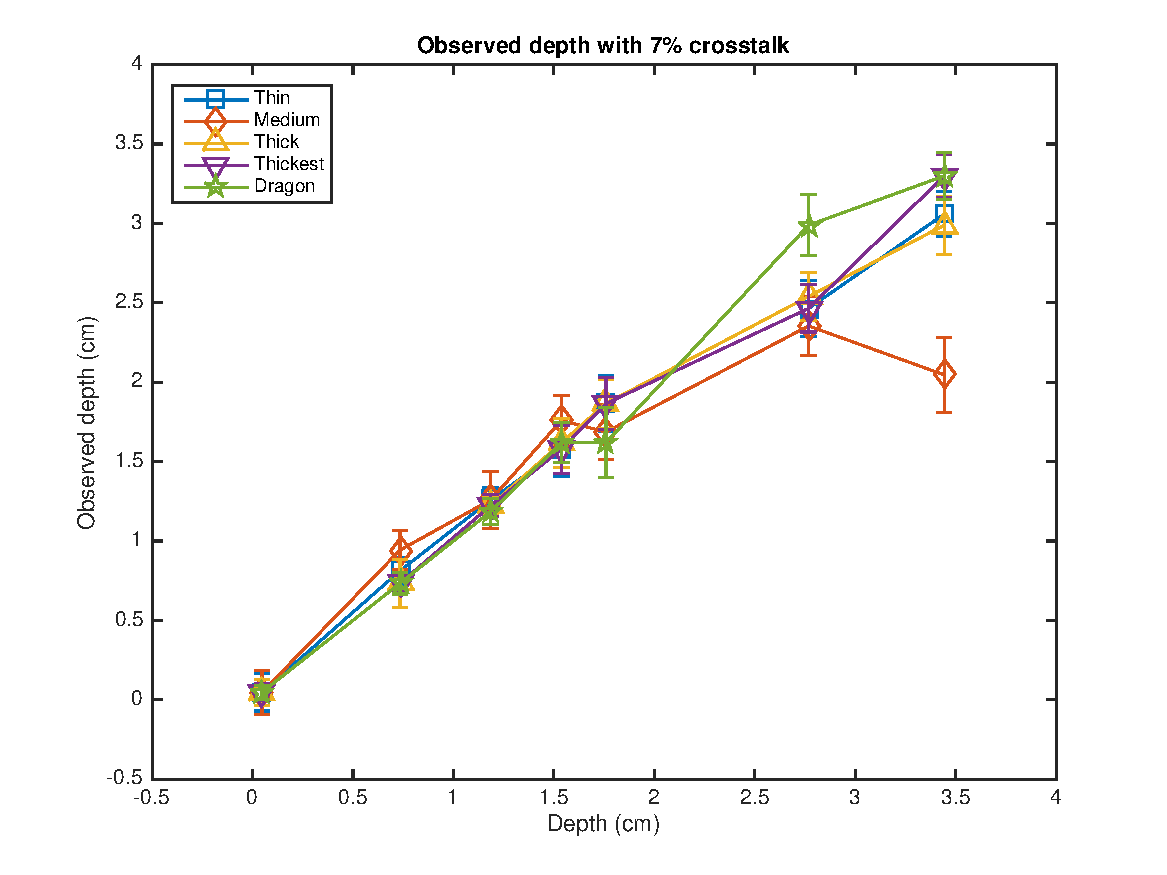
\includegraphics[width=0.9\textwidth]{./Template_Figures/a_crosstalk_7}
    \caption{Abscissa shows the observed depth when 7\% crosstalk is present. The error bars indicate $\pm$ 1 standard error.\label{fig:a_crosstalk_7}}
\end{figure}

\begin{figure}[H]
\centering
    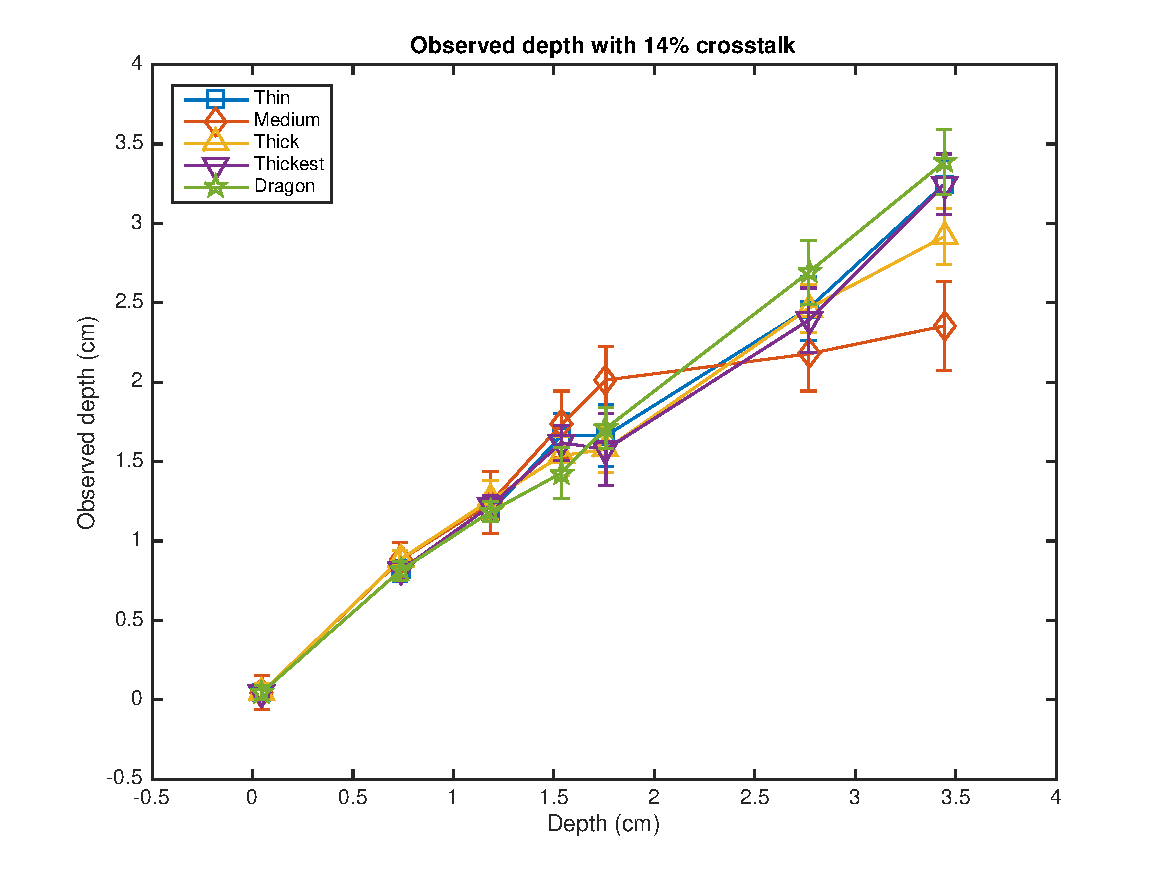
\includegraphics[width=0.9\textwidth]{./Template_Figures/a_crosstalk_14}
    \caption{Abscissa shows the observed depth when 14\% crosstalk is present. The error bars indicate $\pm$ 1 standard error.\label{fig:a_crosstalk_14}}
\end{figure}

\section {Discussion}
\subsection{Stereo}
is edge playing a role?
the degraded depth increased as the crosstalk and the disparity increase. thin objects are affected the most even if the ghost is not completely separated.
why does the degradation start at 1.76 cm for all objects other than thin cylinder where it starts at 1.13 cm?
make a table of ghost separation and discuss at what percentage the depth degradation occurs.
discuss why the ghost are always diplopic and why it can cause hindrance. (finind peaks can be problamatic).
discuss the correlation theory and why it fails here.
what could be going on in HVS windowed correlation etc? or averaging of peaks.
what crosstalk level is ok according to these results?

\subsection{Automultiscopic}


